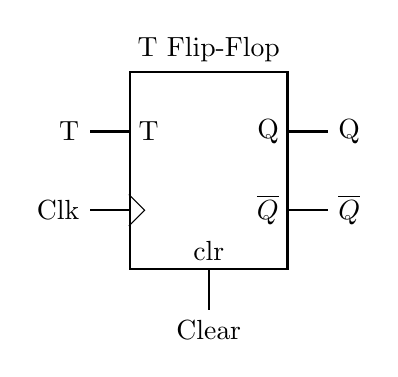
\begin{tikzpicture}
    \node [draw, minimum width=2cm, minimum height=2.5cm, thick] (box) {};
    
    % Input T
    \draw [thick] (box.west) ++(0, 0.5) coordinate (t_in) -- ++(-0.5, 0) node[anchor=east] {T};
    \node [anchor=west] at (t_in) {T};
    
    % Input Clock
    \draw [thick] (box.west) ++(0, -0.5) coordinate (clk_in) -- ++(-0.5, 0) node[anchor=east] {Clk};
    \draw (box.west) ++(0, -0.3) -- ++(0.2, -0.2) -- ++(-0.2, -0.2); % Clock triangle
    
    % Input Reset (Asynchronous clear)
    \draw [thick] (box.south) -- ++(0, -0.5) node[anchor=north] {Clear};
    \node [anchor=south] at (box.south) {clr};
    
    % Output Q
    \draw [thick] (box.east) ++(0, 0.5) coordinate (q_out) -- ++(0.5, 0) node[anchor=west] {Q};
    \node [anchor=east] at (q_out) {Q};
    
    % Output Qn
    \draw [thick] (box.east) ++(0, -0.5) coordinate (qn_out) -- ++(0.5, 0) node[anchor=west] {$\overline{Q}$};
    \node [anchor=east] at (qn_out) {$\overline{Q}$};
    
    % Label
    \node [above] at (box.north) {T Flip-Flop};
\end{tikzpicture}
